

%%%%%%%%%%%%%%%%%%%%%%%%%%%%%%%%%%%%%%%%%%%%%%%%%%%
%%%%%%%%%%%%%%%%%%%%%%%%%%%%%%%%%%%%%%%%%%%%%%%%%%%
%%%%%%%%%%%%%%%%%%%%%%%%%%%%%%%%%%%%%%%%%%%%%%%%%%%
\documentclass{llncs}
\usepackage[spanish]{babel}
\usepackage[utf8]{inputenc}
\usepackage{graphicx}
\usepackage{amsmath}



\begin{document}
\title{Rényi Map}

\subtitle{Resumen}




%For multiple authors:
\author{Marcos Daniel Calderón Calderón}


%If using runnningheads you can abbreviate the author name on even pages:
%\authorrunning{abbreviated author name}
%and you can change the author name in the table of contents
%\tocauthor{enhanced author name}

%For a single institute
\institute{Centro de Investigación en Matemáticas \\ \email{marcos.calderon@cimat.mx}}

\maketitle

\begin{abstract}
Resumen sobre un generador congruencial, se incluyen algunos ejemplos.
\end{abstract}

\section{Introducción.}

La generación de números pseudoaleatorios es una custión muy importante en muchas aplicaciones, como la criptografía, simulación estocástica, prueba de circuitos digitales y sistemas de telecomunicaciones. En muchas de estas aplicaciones,los números aleatorios son generados por medio de generadores de números pseudoaleatorios (PRNGs)  los cuales son máquinas de estados finitos que evolucionan libremente  al ser inicializados por una semilla especial, elegia dentro del espacio de estados. El propósito de un PRNG es emular, dentro de un periodo, una fuente de información que emite símbolos independientes entre sí y que además están igualmente distribuidos.
La arquitectura básica de un PRNG  incluye un bloque de memoria que tiene $n$ flips flops que almacenana el estado presente $k_{z}$, una  lógica de formación de entrada  que se utilizará para evaluar el siguiente estado $k_{z+1}$ de acuardo a una relación recursiva $k_{z+1}$= $f(k_{z})$, y una lógica de formación de salida, la cual evalúa la saluda actual $OUT_{z}= g(k_{z})$. Típicamente, por medio de una normalización apropiada, la función $g$ nos da números que deben de pertenecer al intervalo unitario [0,1). Cuando la salida $OUT_{i}$ consigue valores que pertenecen a ${0,1}$, el PRNG es un generador de bits pseudoaleatorio. 

Para la definición de un a lógica de formación de entrada $f$, las transformaciones lineales son una elección muy popular. Un ejemplo es el siguiente generador recursivo 

\begin{equation}
k_{z+1}=  (a_{1}k_{z}+ a_{2}k_{z-1}+ ... + a_{m}k_{z-m+1}+c) \quad mod \quad M
\end{equation}

La expresión (1) es utilizada en muchos generadores importantes, por ejemplo, el generador lineal congruencial (LCG) y la familia de los  linear feedback shift registers (LFSR). El uso de recurrencias lineales  permitidas para un PRNG traer beneficios: son muy eficientes en términos de alto rendimiento y baja complejidad en hardware y software. PNRG basados en recurrencias lineales  normalmente generan secuencias cuya aleatoriedad es afectada por alguna regularidad no deseada, y por lo tanto no adecuado para una amplia clase de aplicaciones.

A continuación se muestran los resultados de un ejemplo de un generador lineal congruencial de la forma $s_{i}= (as_{i-1}+b)mod M$ donde $s_{0}=0$, $a=3$, $b-5$ y $M=31$ ~\ref{sample-table}.

\begin{table}[t]
\caption{Resultados de un generador lineal congruencial}
\label{sample-table}
\begin{center}
\begin{tabular}{ll}
\multicolumn{1}{c}{\bf Interación }  &\multicolumn{1}{c}{\bf Valor de s}
\\ \hline \\

1 &  0\\
2  & 5\\
3  & 20\\
4 &  3\\
5  & 14\\
6  & 16\\
7  & 22\\
8  & 9\\
9 &  1\\
10  & 8\\
11 &  29\\
12 & 30\\
13 & 2\\
14 & 11\\
15 & 7\\
16 & 26\\
17 & 21\\
18 & 6\\
19 & 23\\
20 & 12\\
21 & 10\\
22 & 4\\
23 & 17\\
24 & 25\\
25 & 18\\
26 & 28\\
27 & 27\\
28 & 24\\
29 & 15\\
30 & 19\\
\end{tabular}
\end{center}
\end{table}


También se pueden utilizar recurrencias no lineales para la definición de un PRNG, su principal ventaja es que este tipo de generadores no sufren de  problemas de periodicidad de los valores; sin embargo,  su copmplejidad computacional es mayor.

En tiempos mas recientes, se han investigado sistemas dinámicos caóticos para generar secuencias de números pseudoaleatorios. En este tipo de PRNG, la lógica de formación de entrada es obtenida al digitalizar un mapa no lineal de la forma $\phi:  \Lambda \longrightarrow \Lambda$, donde $\Lambda \subset \mathbf{R}$ es un atractor en un sistema caótico. La digitalización de un sistema caótico  se logra al discretizar el espacio de estados $\Lambda$ y recurrir a una aproximación numérica  del mapa $\phi$.
\section{Criterio común para la evaluación de un generador de números pseudoaleatorios.}


Los generadores de números pseudoaleatorios (PRNG, siglas en inglés) operan sobre dominios finitos, por lo tanto, las secuencias de números son  siempre eventualmente periodicas. Normalmente, el tamaño del período $\lambda$ es menor o igual al espacio de cardinalidad $2^{n}$, y en general, este depende de la semilla inicial $k_{0}$. Dependiendo de la semilla inicial, varios tipos de trayectorias pueden ser generadas por un PRNG.

Como la salida de un PRNG depende de la logica de formación de salida, una mala elección de una función $g$ puede dar secuencias con un período más corto que el período del estado interno. De cualquier manera, la función $g$ debe asegurar buenas propiedades estadísticas de las secuencias generadas, debe también preservar la longitud del período. La periodicidad de la salida es uno de los principales aspectos que revelan la no aleatoriedad del subestpacio. 

En general, una secuencia aleatoria generada por una fuente debe de satisfacer la hipótesis nula $H_{0}:$  ''Los símbolos de salida son independientes entre sí y representan una distribución uniforme''. Es obvio que para cualquier secuencia generada por un PRNG determinístico, $H_{0}$ es falsa a priori.

El grado de aleatoriedad de una secuencia pseudoaleatoria es evaluada por medio de exámenes estadísticos que verifican la hipótesis nula $H_{0}$. Existen muchos exámenes de este tipo, por ejemplo: NIST, Diehard.


\section{Renyi map digitalizado.}

Los PRNG basados en la digitalización de los mapas caóticos, realizan una versión discreta de un mapa contínuo $\phi$, se avelúa $\phi$ y se representa el estado con valor real $x$ con una precisión finita de n bits. Incluso aunque el mapa $\phi$ y la representaci[on de el estado digitalizado $x$ puede ser arbitrariamente elegido, las soluciones que requieren implementaciones de baja complejidad de hardware son las preferidas. Desde este punto de vista, mapas caóticos lineales a trozos son buenos candidatos para implementar la lógica de la digitalización, porque la estructura analítica implica operaciones matemáticas simples. 

El mapa caótico Rényi es definido de la siguiente manera:

\begin{equation}
\begin{aligned}
\phi_{\beta}:[0,1) \longrightarrow [0,1) \quad \textbf{donde}\\
\phi_{\beta}(x)=(\beta \cdot x)\quad  mod \quad 1
\end{aligned}
\end{equation}

donde $1 < \beta \in \mathbf{R}$, y para cualesquiera números reales no negativos: $a, b, a \quad mod \quad b= a- \lfloor a/b \rfloor b$.

Además, definimos $\tilde{x}$ como un estado digitalizado, esto es: una representación de punto fijo de el sistema tal que 
\begin{equation}
\begin{aligned}
\tilde{x} \in \mathbf{Q}: \quad \tilde{x}= \frac{k}{2^{n}}, \quad k \in \mathbf{N}, \quad k < 2^{n}.
\end{aligned}
\end{equation}

De acuerdo a la ecuacion anterior, el estado digitalizado es un número racional en [0,1), y la cardinalidad del espacio del estado discretizado es de $2^{n}$.

Para la precisión finita de (2), la estrategia de aproximación por truncamiento es considerada, esto es:
\begin{equation}
\begin{aligned}
\tilde{\phi}_{\beta}(\tilde{x})= (\beta \cdot \tilde{x})_{tr} \quad mod \quad 1=
\lfloor (2^{n}\cdot \beta \cdot \tilde{x} )\quad mod \quad 2^{n}  \rfloor \cdot 2^{-n}.
\end{aligned}
\end{equation}

Como (4) debe ser implementado en máquinas de estado finito, $\beta$ puede ser en general cualquier número racional más grande que 1 y cuya representación binaria requiere un número finito de dígitos. Por medio del isomorfismo $k = \tilde{x}2^{n}$, el estado discretizado definido en (3) puede ser relacionado con el conjunto de números naturales 

\begin{equation}
\begin{aligned}
\Delta _{n}= \lbrace k \in \mathbf{N}, 0 \leq k < 2^{n}  \rbrace
\end{aligned}
\end{equation}

y una función  $f: \Delta_{n} \rightarrow \Delta_{n} $ puede ser definida como 
\begin{equation}
\begin{aligned}
f(k)= 2^{n}\tilde{\phi}_{\beta}(2^{-n}k)=\lfloor \beta \cdot k \quad mod \quad 2^{n}  \rfloor \\
=\lfloor  \beta \cdot k  \rfloor \quad 2^{n}.
\end{aligned}
\end{equation}


Desde un punto de vista dinámico, la función $f$ es equivalente a (4) y en lo siguiente, nos referiremos a (6) para la definición de la lógica de formación de entrada de los PRNGs propuestos en este resumen. Más que eso, si $k = 2^{n} \cdot \tilde{x} = 2^{n} \cdot \sum_{j=1}^{n} b_{j}2^{-j} $, la expresión $(b_{1}b_{2}...b_{n})_{2}$ es el valor del estado del PRNG alamcenado en el registro del enésimo bit.

A continuación, se muestra una gráfica los valores generados con la ecuación (6).
\begin{figure}[h!]
\centering
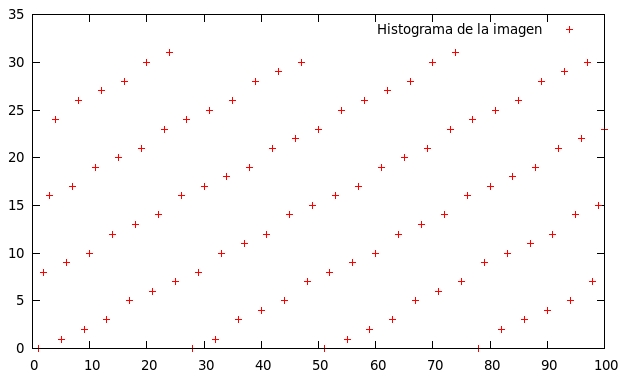
\includegraphics[width=8cm]{a.jpg}
\caption{Rényi map.}
\label{rbasico}
\end{figure}


\subsection*{La estructura analítica de la logica de formación de salida.}
El parámetro racional $\beta$ puede ser escrito como la suma de una parte entera $b$ y una parte fraccional $\gamma$. Por lo tanto, (6) puede ser escrito de la siguiente manera: 
\begin{equation}
\begin{aligned}
f(k)= (bk + \lfloor \gamma \cdot k  \rfloor)\quad mod \quad 2^{n}.
\end{aligned}
\end{equation}

Si $\gamma >0$, la expresión previa puede ser reescrita como:

\[f(k)=
\left\{
\begin{array}{rcl}
(bk) mod 2^{n}, & \mbox{si} & 0 \geq k \geq  \frac{1}{\gamma}\\
(bk+1) mod 2^{n}, & \mbox{si} & \frac{1}{\gamma} \geq k \geq  \frac{2}{\gamma}\\
. \\
. \\
. \\
(bk+p_{max}) mod 2^{n}, & \mbox{si} & \frac{p_{max}}{\gamma} \geq k \geq 2^{n}\\
\end{array}
\right. \]

donde $p_{max}= \lfloor (2^{n}-1)\gamma \rfloor$ En la siguiente figura se puede ver un ejemplo de mapa con $\beta= 8.32125$ y $n=5$.



\section{Periodo de los NLCGs propuestos.}

A la hora de observar la fórmula para el Renyi Map, debemos de evitar el valor de $k=0$ porque esto es un valor fijo, y debe ser excluido a la hora de hacer una elección para la semilla inicial.
El máximo periodo que se puede lograr es de  $\lambda_{max}=2^{n}-1$. En este caso, se está trabajando con $n=32$. 

Una cosa interesante a descubrir es la manera en cómo los valores de $i, j, n$ deben de ser para obtener un periodo máximo. EL hecho de truncar valores decimales en la fórmula para el Renyi Map hace difícil elegir valores adecuados para los parámetros que se mencionan.

Si un PRNG como el Renyi Map tiene un periodo máximo, entonces es invertible: el estado $k=0$ es un punto aislado y cada estado en la óebira debe tener un simple predecesor. Una proposición importante es la siguiente:

El mapa Renyi Map es invertible si $i=j$. Esto reduce la cardinalidad de los mapas posibles de $n2^{n}$ a $2^{n}-1$.



\section{Resultados.}
A continuación, vamos a encontrar el período de los siguientes sistemas de Renyi Map:

\begin{enumerate}

\item $n= 32$, $i,j =3, q=3$ Al sustituir los parámetros anteriores, obtenemos la siguiente expresión.

\begin{equation}
f(x+1)=  \left( 1610612736(k) + \lfloor \frac{k}{8} \rfloor   \right) \mod(2^{32})
\end{equation}

Si convertimos el parámetro de la multiplicación a hexadecimal, obtenemos la siguiente expresión:
expresión.

\begin{equation}
f(x+1)=  \left(  60000000(k) + \lfloor \frac{k}{8} \rfloor   \right) \mod(2^{32})
\end{equation}

No se obtuvieron buenos resultados, se llega al punto fijo $k=0$ rápidamente.




\item $n= 32$, $i,j =4, q=9$ Al sustituir los parámetros anteriores, obtenemos la siguiente expresión.

\begin{equation}
f(x+1)=  \left(  2415919104(k) + \lfloor \frac{k}{16} \rfloor   \right) \mod(2^{32})
\end{equation}

Si convertimos el parámetro de la multiplicación a hexadecimal, obtenemos la siguiente expresión:
expresión.

\begin{equation}
f(x+1)=  \left(  90000000(k) + \lfloor \frac{k}{16} \rfloor   \right) \mod(2^{32})
\end{equation}

Sin embargo, no se obtuvieron buenos resultados, se llega al punto fijo $k=0$ rápidamente.




\item $n=32$, $i,j =3, q=1$ Al sustituir los parámetros anteriores, obtenemos la siguiente expresión.

\begin{equation}
f(x+1)=  \left( 536870912(k) + \lfloor \frac{k}{8} \rfloor   \right) \mod(2^{32})
\end{equation}

Si convertimos el parámetro de la multiplicación a hexadecimal, obtenemos la siguiente expresión:
expresión.

\begin{equation}
f(x+1)=  \left(  20000000(k) + \lfloor \frac{k}{8} \rfloor   \right) \mod(2^{32})
\end{equation}

No se obtuvieron buenos resultados, se llega al punto fijo $k=0$ rápidamente.
\end{enumerate}

De acuerdo a lo anterior, si tomamos los mismos parámetros del paper para $n=32$, no se obtienen los resultados esperados. Entonces, 


\subsubsection*{Referencias}


%The bibliography, done here without a bib file
%This is the old BibTeX style for use with llncs.cls
\bibliographystyle{splncs}

%Alternative bibliography styles:
%the following does the same as above except with alphabetic sorting
%\bibliographystyle{splncs_srt}
%the following is the current LNCS BibTex with alphabetic sorting
%\bibliographystyle{splncs03}
%If you want to use a different BibTex style include [oribibl] in the document class line

\begin{thebibliography}{1}
%add each reference in here like this:
\bibitem[RE1]{reference1}
 T. Addabbo, M. Alioto, A. Fort, A. Pasini, S. Rocchi, V. Vignoli
 A class of Maximum-Perior Nonlinear Congruential Generators Derived From the Rényi Chaotic Map.
 2007, IEEE 
\end{thebibliography}

\end{document}

